\documentclass[a4paper]{article}
\usepackage[UTF8,fontset=none]{ctex}
\usepackage[a4paper,margin=1in]{geometry}
\usepackage{graphicx,float,booktabs,longtable,amsmath,amssymb}
\usepackage[dvipsnames,table]{xcolor}
\usepackage{hyperref,fancyhdr,lastpage,enumitem,tikz}
\usetikzlibrary{arrows.meta,positioning,shapes.geometric}
\setCJKmainfont{Songti SC}
\setCJKsansfont{Songti SC}
\setlength{\parindent}{2em}
\hypersetup{hidelinks}
\pagestyle{fancy}
\fancyhf{}
\fancyhead[L]{OS 功能挑战赛 Proj59（决赛）}
\fancyhead[C]{SLIM-ARC}
\fancyhead[R]{中山大学}
\fancyfoot[C]{第 \thepage 页，共 \pageref{LastPage} 页}
\title{SLIM-ARC：面向内存受限端侧系统的\\MoE 推理运行时设计与跨设备评测}
\author{欧阳易芃\quad 马福泉\quad 刘昊\\指导教师：赵帅\quad 张献伟\\中山大学}
\date{2026 年 8 月}

\begin{document}
\begin{titlepage}
  \centering
  
\includegraphics[width=9cm]{figures/SYSULogo.png}\par
  \vspace{3em}
  {\Large 2026 年全国大学生计算机系统能力大赛\par}
  \vspace{0.8em}
  {\Large 操作系统设计赛（全国）OS 功能挑战赛道\par}
  \vspace{3em}
  {\fontsize{25pt}{31pt}\bfseries SLIM-ARC：面向内存受限端侧系统的\par}
  \vspace{0.4em}
  {\fontsize{25pt}{31pt}\bfseries MoE 推理运行时设计与跨设备评测\par}
  \vspace*{\fill}
  {\large 赛题：Proj59 内存受限环境的大语言模型推理优化\par}
  \vspace{1.5em}
  {\large 组员：欧阳易芃、马福泉、刘昊\par}
  {\large 指导教师：赵帅、张献伟\par}
  {\large 学校：中山大学\par}
  \vspace*{\fill}
  {\large 2026 年 8 月\par}
\end{titlepage}

\tableofcontents
\newpage

\section{引言}

大语言模型的参数规模和上下文长度持续增长，模型权重、KV cache、临时张量与操作系统页缓存共同构成了显著的运行时内存压力。MoE 模型只为每个 token 激活少量专家，降低了实际计算量；但完整权重仍需存放在本地介质，稀疏计算也不会自动转化为稀疏物理内存。对于文件大小 48.41\,GB 的 Qwen3-Next-80B-A3B Q4\_K\_M，2--8\,GiB 的端侧环境无法让全部权重常驻，推理性能取决于运行时如何组织映射、预取、回收、专家驻留与 KV cache。

SLIM-ARC 面向 CPU 为主的端侧设备，将模型访存视为操作系统、运行时和模型结构共同决定的问题。系统不修改权重与 Router 语义，而是在 llama.cpp 的 mmap 路径上增加阶段感知的页建议、分层预取、专家反馈闭环、压力感知预算与 KV 管理。统一调度器在 Prefill 和 Decode 之间切换策略，并依据设备的内存压力、存储介质和缓存状态选择合适配置。

本文的主要贡献如下。
\begin{itemize}[leftmargin=3em]
  \item 提出阶段感知的权重访问控制方法，将 mmap、CPU repack、页建议、层级预取和设备存储特性纳入统一运行时。
  \item 设计 Router 反馈驱动的 MoE 专家管理闭环，以轮次标识关联预测和事实，并通过安全页范围、热度、压力与预算控制专家页面。
  \item 实现模型所有权的运行时、租约化访问、有界队列和统一指标，使后台任务与模型映射具有明确生命周期。
  \item 在 x86/WSL、RK3588、Raspberry Pi 5 和 Mac/Colima 上完成跨设备评测。WSL 8\,GiB 同合同实验将 80B Decode 从 0.08 提升至 0.43\,token/s；48.41\,GB 模型能够在 2\,GiB、no-swap 条件下推理；RK3588 3\,GiB 下 Decode 从 0.70 提升至 2.21\,token/s。
\end{itemize}

\newpage
\section{背景、相关工作与研究动机}

\subsection{端侧推理的内存层次}

端侧推理的内存需求由权重、KV cache、计算临时量和页缓存共同组成。mmap 只建立虚拟地址映射，首次访问仍需通过 major page fault 从存储读取。Linux cgroup v2 的 \texttt{memory.max}、\texttt{memory.current} 与 \texttt{memory.peak} 为实验提供了可复现的物理内存边界。\texttt{madvise} 与 \texttt{posix\_madvise} 可以表达 SEQUENTIAL、NORMAL、RANDOM、WILLNEED 和 DONTNEED 等访问建议，为运行时控制 readahead 与页缓存提供了标准接口。

MoE Router 根据 token 表征选择 top-$k$ 专家。稀疏专家访问形成了潜在的小工作集，但选择结果产生之前只能依赖历史、跨层或在线转移信息进行预测。专家切片还可能与相邻专家共享边界页，因此页面回收必须验证张量布局、专家编号、地址溢出和完整内部页范围。

\subsection{相关工作}

FlexInfer 研究端侧张量卸载、保留和异步预取；PowerInfer-2 通过细粒度缓存与预取支撑手机推理；KTransformers 将 MoE 热冷专家映射到 CPU/GPU 异构执行。FlashAttention、PagedAttention 与 StreamingLLM 分别从 Attention I/O、KV 分页和长序列窗口控制降低运行时开销。SLIM-ARC 吸收这些系统的预算化和异步化思想，但主要面向 CPU-only、POSIX mmap 与普通端侧存储，使机制在没有专用加速核或直接存储通路时仍可工作。

\subsection{研究动机}

本项目聚焦四个相互关联的问题：第一，Prefill 的大范围扫描与 Decode 的稀疏复用需要不同页策略；第二，专家预测必须与实际 Router 选择关联，才能管理投机 I/O；第三，普通权重、专家和 KV cache 必须共享统一资源预算；第四，后台预取线程必须服从模型映射的生命周期。对应地，SLIM-ARC 采用阶段控制器、专家反馈闭环、压力准入和模型所有权运行时，形成从访问预测到资源结算的完整链路。

\newpage
\section{SLIM-ARC 系统设计}

\subsection{总体架构}

图\ref{fig:architecture}展示系统的五层结构。模型层保留原始 GGUF 权重和 Router 语义；运行时层识别阶段并生成页访问动作；操作系统层执行 mmap、页建议与 cgroup 约束；存储层承载远大于物理内存的模型文件；指标层记录吞吐、缺页、I/O、预算和专家状态。统一调度器连接普通权重、专家与 KV 路径，避免各模块独立扩大工作集。

\begin{figure}[H]
  \centering
  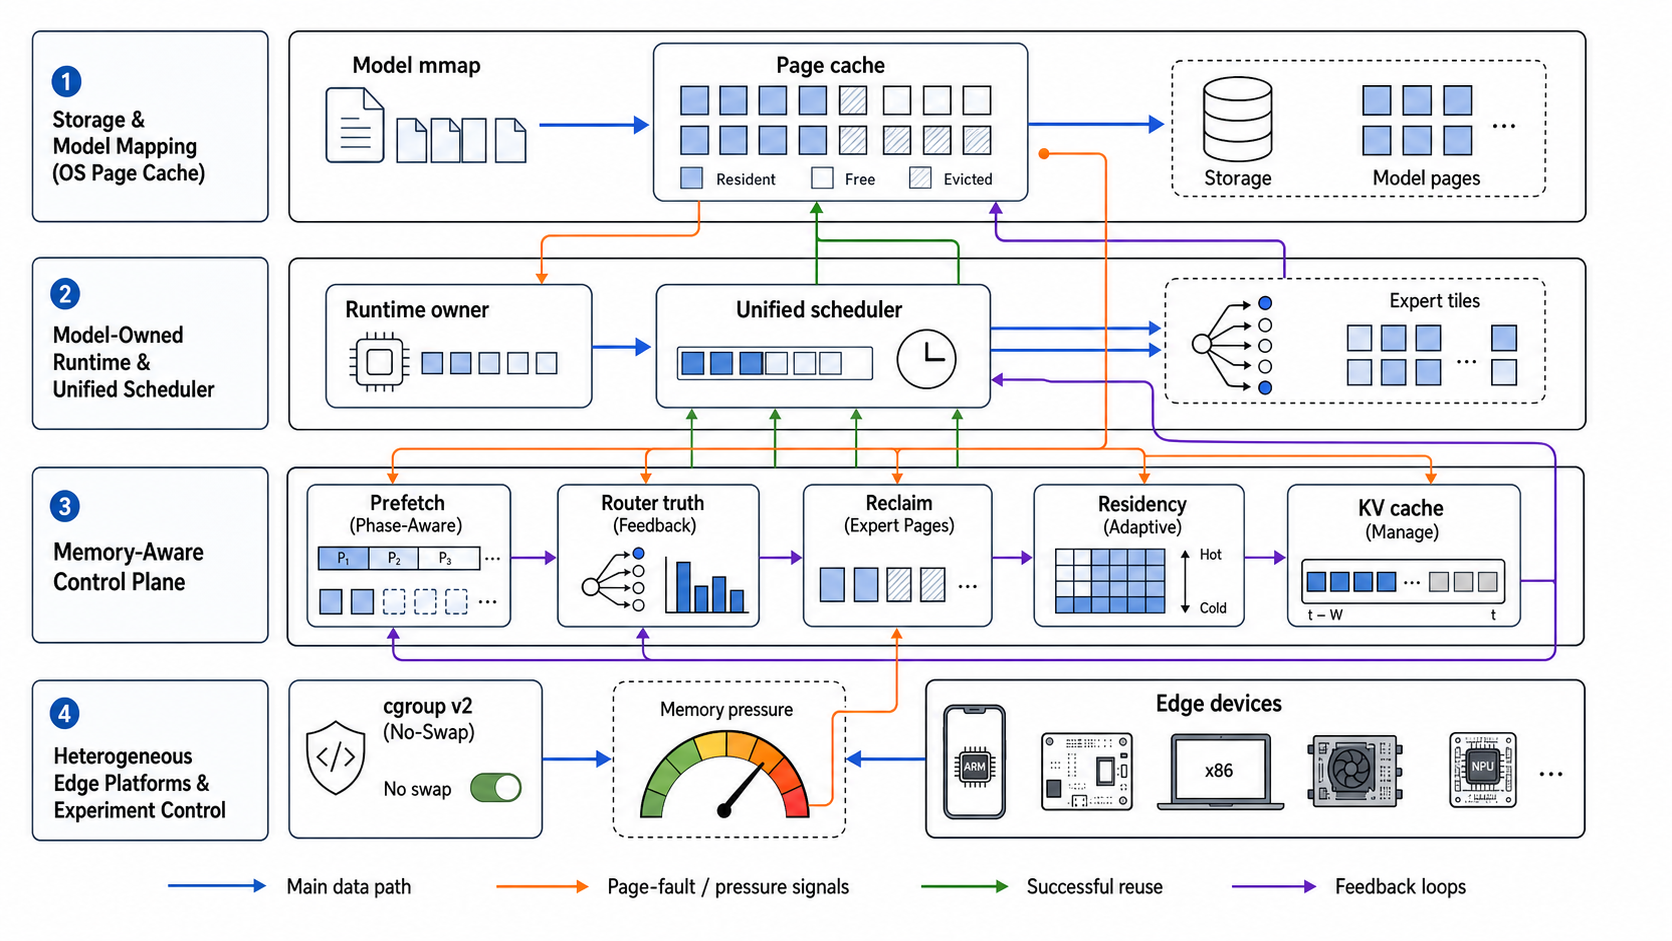
\includegraphics[width=0.98\textwidth]{figures/system_architecture.png}
  \caption{SLIM-ARC 的分层系统架构。}
  \label{fig:architecture}
\end{figure}

\subsection{阶段感知页访问}

系统将执行划分为模型加载、Prefill、普通 Decode 和 MoE Decode。Prefill 按层扫描较大的权重集合，优先使用顺序预读并提前有限层数；Decode 重复访问少量活跃页面，预取窗口随预算收缩；MoE Decode 进一步利用 Router 产生的稀疏专家集合。策略切换只改变访问提示，不改变张量内容与计算顺序。

页建议采用 best-effort 语义。所有地址先转换为页边界范围，长度和地址运算进行溢出检查；建议调用在状态锁之外执行，避免慢系统调用阻塞 Router 与调度线程。运行时记录成功建议字节而非请求字节，使指标能够对应实际内核动作。

\subsection{MoE 专家预测与反馈闭环}

系统支持 temporal、跨层 Router 和热度候选。每次专家预取分配不可复用的 generation token，预取成功的专家编号和字节数以 token 为键保存；实际 Router 结果到达后只结算一次。图\ref{fig:router}展示跨层预测路径：第 $N$ 层 Router 的选择转化为下一层候选，在第 $N+1$ 层计算之前向内核表达 WILLNEED。

\begin{figure}[H]
  \centering
  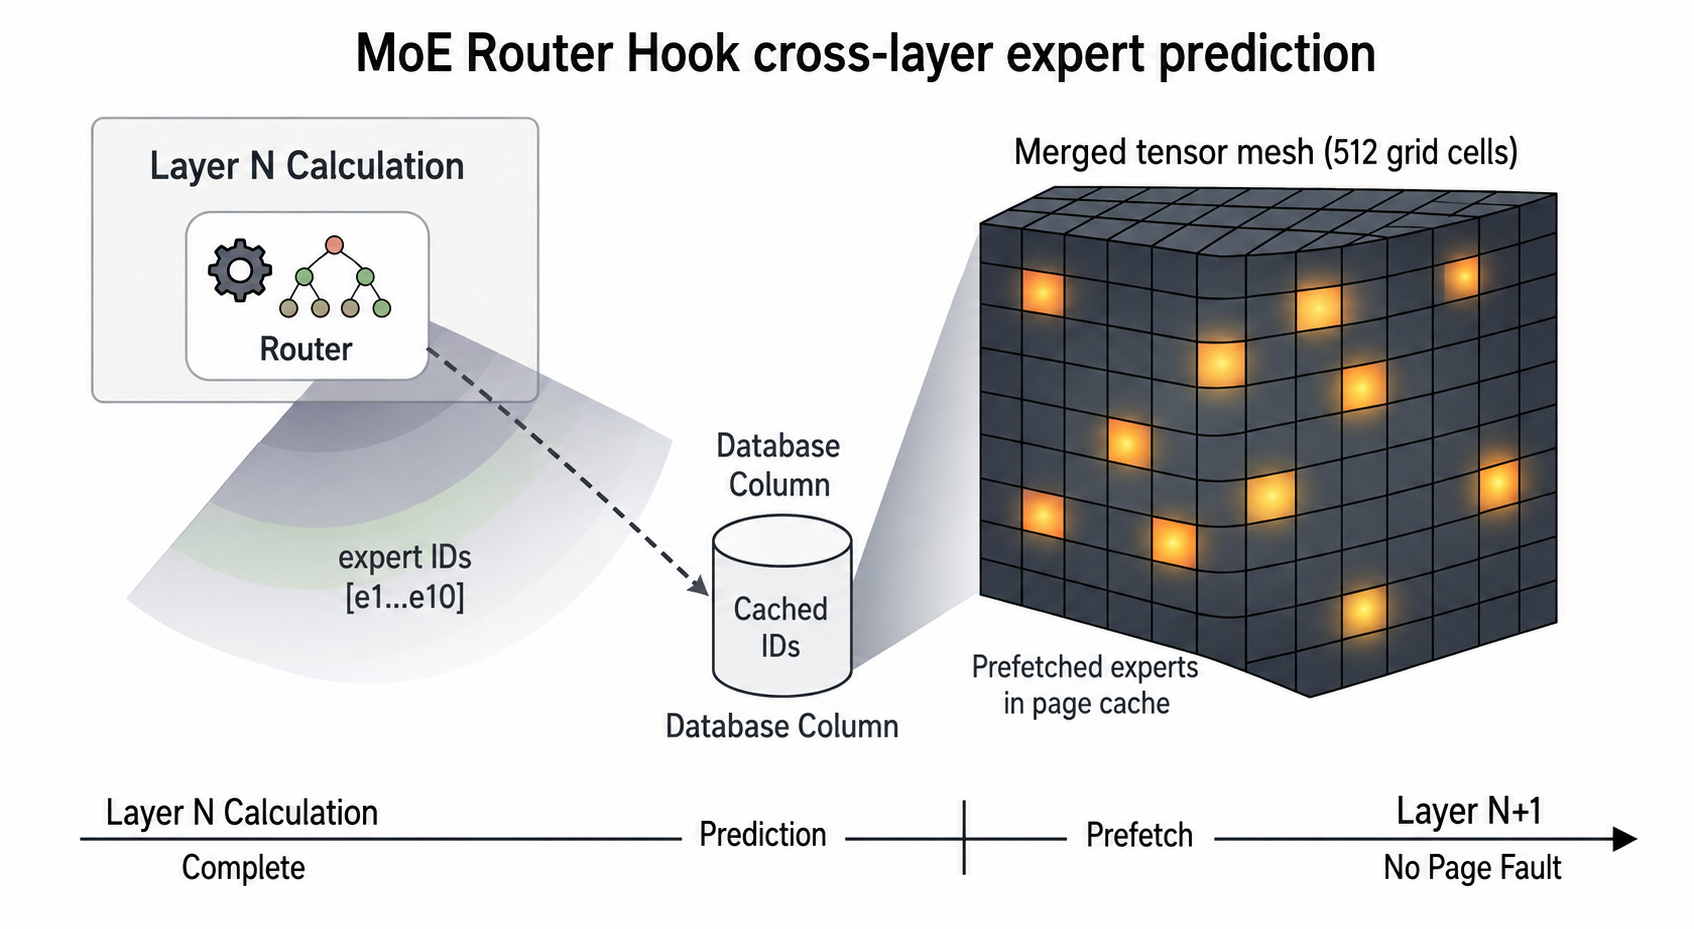
\includegraphics[width=0.98\textwidth]{figures/moe_router_hook.png}
  \caption{跨层 Router 预测与专家页面预取。}
  \label{fig:router}
\end{figure}

事实结算后，运行时更新专家热度、命中和浪费统计。对未选择专家，只对完全位于切片内部的页面生成 DONTNEED 计划；首尾共享页保持不动。回收和驻留均受特性开关与预算约束，因此核心推理路径能够独立运行。

\subsection{压力感知驻留与统一预算}

压力控制器以 cgroup 当前使用量与上限计算状态，并使用滞回避免阈值附近频繁切换。正常压力下按稳定专家、时间相邻专家和热专家排序；较高压力下只保留确定性较强的稳定集合；临界压力下停止新增驻留。浪费比例使用整数 EWMA 平滑，专家热度定期衰减，避免早期请求永久支配缓存。

统一预算先扣除安全预留，再分配给普通权重、专家和 KV 路径。所有加法、乘法和字节累计都使用饱和或显式检查；压力信息缺失时选择保守配置。该设计使内存上限成为真正的共享约束，而不是多个模块各自解释的参数。

\subsection{KV cache 与长上下文}

KV 路径结合低比特表示、attention sink 与最近窗口。图\ref{fig:kv}中，固定保留 sink token 与最近窗口，中间区域按策略释放或映射到临时文件，使 KV 占用从上下文长度线性增长转为与 sink 和窗口大小相关。权重页与 KV 预算由同一调度器协调，从而在长上下文下保留模型权重工作集的空间。

\begin{figure}[H]
  \centering
  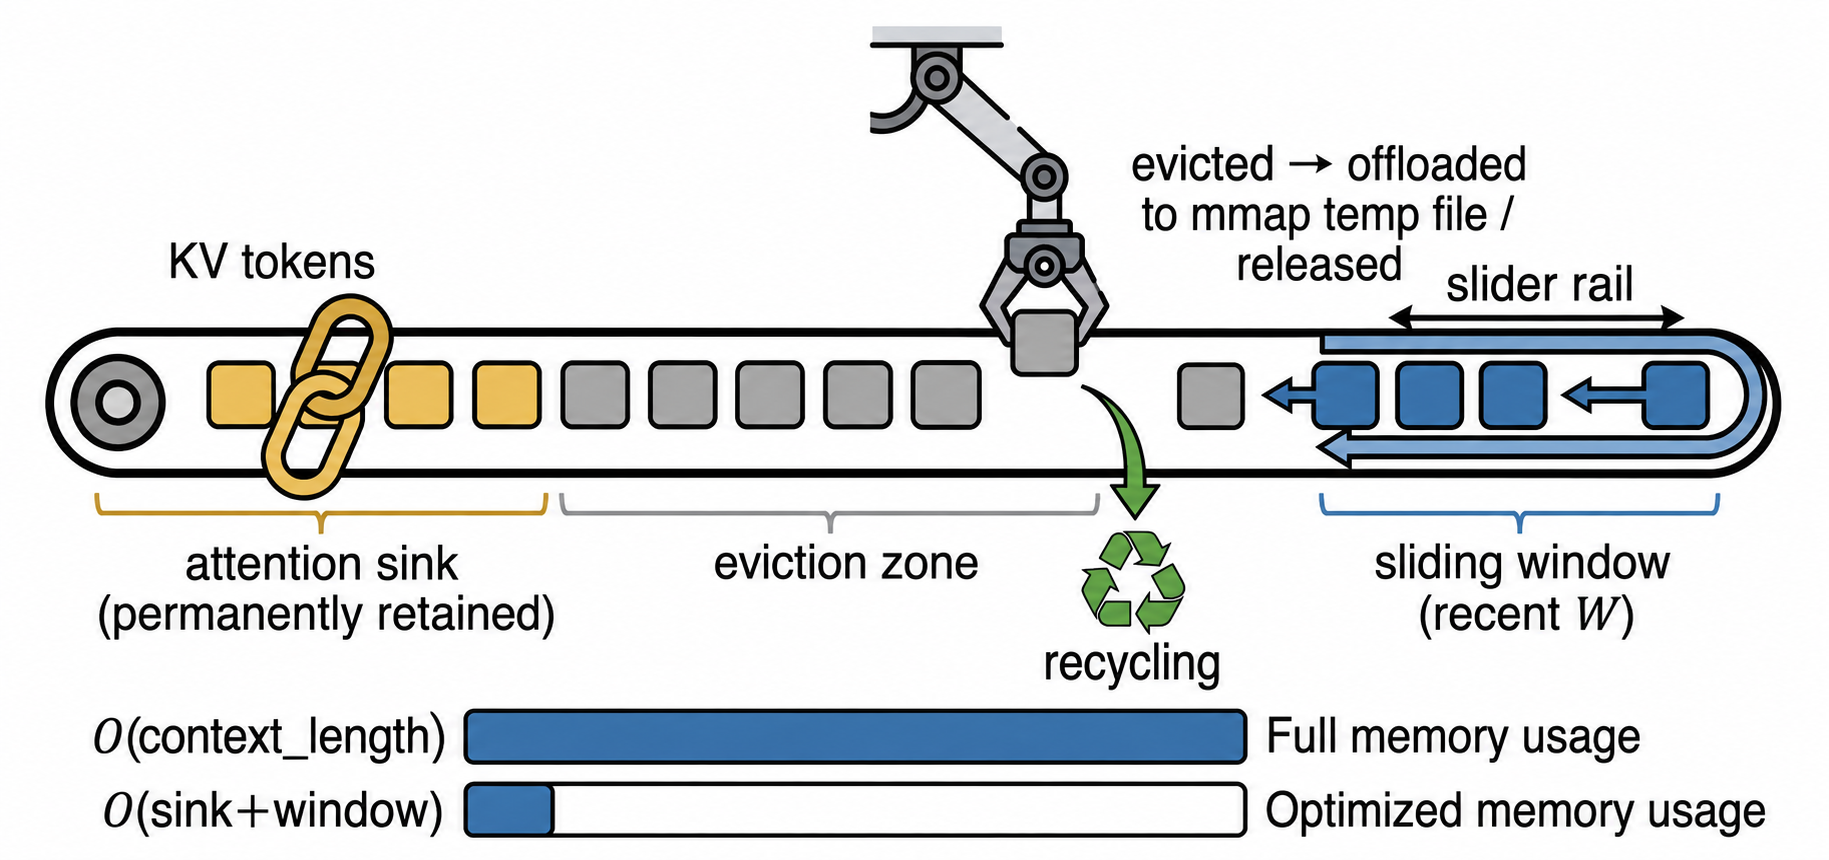
\includegraphics[width=0.96\textwidth]{figures/kv_eviction.png}
  \caption{attention sink、滑动窗口与 KV 页面管理。}
  \label{fig:kv}
\end{figure}

\newpage
\section{系统实现}

\subsection{llama.cpp 集成}

项目以固定 llama.cpp 提交为基线，通过可重复应用的补丁脚本复制独立模块并插入构建目标。模型对象在完成 mapping 转移后创建运行时，运行时内部依次持有预取调度器与统一调度器；析构顺序保证 worker 停止后映射才被释放。图\ref{fig:modules}给出主要模块和调用关系。

\begin{figure}[H]
  \centering
  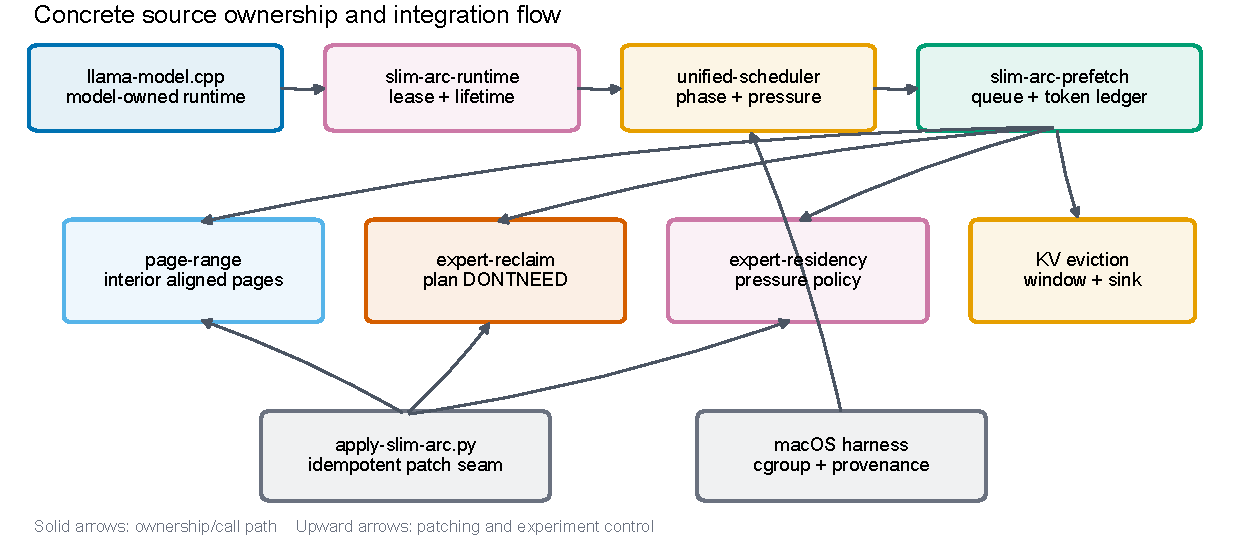
\includegraphics[width=0.98\textwidth]{figures/implementation_module_map.pdf}
  \caption{运行时模块、模型所有权与图执行钩子的实现关系。}
  \label{fig:modules}
\end{figure}

图执行只通过运行时租约访问调度器。租约在模型析构前登记关闭状态，随后等待在途访问退出；任何新请求都会得到空租约。该机制消除了进程全局裸指针与映射地址分离的问题。预取 worker 使用有界请求队列和单调 generation，重复层通知、图失败与无 Router 节点均有确定的终态结算。

\subsection{关键模块}

\begin{longtable}{p{0.29\textwidth}p{0.63\textwidth}}
\toprule
模块 & 职责 \\
\midrule
\texttt{slim-arc-runtime} & 模型所有权、租约、mapping 与张量注册、调度器生命周期 \\
\texttt{slim-arc-prefetch} & 阶段识别、普通权重与专家预取、有界队列、运行时指标 \\
\texttt{slim-arc-unified-scheduler} & 压力采样、共享预算、权重/专家/KV 协调 \\
\texttt{slim-arc-page-range} & 页对齐、内部完整页与溢出安全计算 \\
\texttt{slim-arc-expert-reclaim} & 错误专家集合、回收计划和成功字节统计 \\
\texttt{slim-arc-expert-residency} & 压力状态、浪费 EWMA、热度衰减和确定性准入 \\
\texttt{slim-arc-kv-eviction} & sink、滑动窗口和 KV 页面释放 \\
\bottomrule
\end{longtable}

\subsection{跨设备实现}

x86/WSL 用于建立 Qwen3-Next-80B 的受限内存基线；RK3588 使用 systemd user scope 与 cgroup v2 构造 2.5--5\,GiB 边界，并针对 ARM CPU 与 SSD 调整阶段页建议；Raspberry Pi 5 使用 4\,GiB 内存和 USB/FUSE 存储，重点保留 shared/hot 专家并严格限制投机 I/O；Mac 通过 Colima ARM64 VM、Docker cgroup v2 和 \texttt{swap.max=0} 形成可重复的 2\,GiB、4 vCPU 环境。所有平台保持模型哈希、缓存状态、Prompt/Generation 长度与线程数随实验记录。

\newpage
\section{实验评估与结果分析}

\subsection{实验设置}

主模型为 Qwen3-Next-80B-A3B-Instruct Q4\_K\_M，文件大小 48,410,988,384\,B，SHA-256 为 \texttt{d103b2733ec1012a52d01edda66b7e5c24ae50508c9f99f5297ea459ef3c061a}。主要指标包括 llama-bench Prefill/Decode token/s、完整 wall time、cgroup peak、major faults、文件输入字节、专家建议字节和缓存命中。提升率只在同设备、同模型、同 workload、相同线程与缓存状态内计算。

\begin{table}[H]
\centering
\small
\caption{主要实验平台与目标}
\begin{tabular}{llll}
\toprule
平台 & 资源约束 & 存储 & 主要目标 \\
\midrule
x86/WSL & 8--32\,GiB cgroup & NVMe & 初赛基线与完整优化栈 \\
RK3588 & 2.5--5\,GiB user scope & SSD & 3\,GiB 主实验与动态页建议 \\
Raspberry Pi 5 & 4\,GiB，no-swap & USB/FUSE & 慢存储驻留与 I/O 预算 \\
Mac/Colima & 2\,GiB，4 vCPU，no-swap & APFS/VM & 80B 极限可运行性 \\
\bottomrule
\end{tabular}
\end{table}

\subsection{主实验}

\subsubsection{x86/WSL：初赛核心性能与优化链}

初赛首先在 Intel i9-13900H、32\,GB DDR5、NVMe SSD 和 Ubuntu 22.04/WSL2 环境中建立 80B 推理基线，并使用 cgroup v2 构造 8、16 和 32\,GiB 三档内存。该平台承担两项核心验证：其一，检验 SLIM-ARC 能否在模型文件显著大于内存上限时提高 Decode 吞吐；其二，测量权重量化、缓存容量与 FlashAttention 对不同运行区间的贡献。

表\ref{tab:wsl-limited}给出 8\,GiB 下两组同合同配对结果。\texttt{pp4/tg1} 合同中，SLIM-ARC 将 Prefill 从 0.22 提高到 0.25\,token/s，将 Decode 从 0.08 提高到 0.43\,token/s；Decode 提升 437.5\%。在较长的 \texttt{pp16/tg4} 合同中，Decode 从 0.08 提高到 0.29\,token/s，提升 262.5\%。两组实验均只在相同内存、模型、Prompt/Generation 长度和缓存条件内计算提升率。

\begin{table}[H]
\centering
\small
\caption{WSL 8\,GiB 下的同合同 80B 配对结果}
\label{tab:wsl-limited}
\begin{tabular}{llrrl}
\toprule
合同 & 配置 & Prefill & Decode & Decode 提升 \\
\midrule
pp4/tg1 & baseline & 0.22 & 0.08 & reference \\
pp4/tg1 & SLIM-ARC & \textbf{0.25} & \textbf{0.43} & \textbf{$+437.5\%$} \\
pp16/tg4 & baseline & -- & 0.08 & reference \\
pp16/tg4 & SLIM-ARC & -- & \textbf{0.29} & \textbf{$+262.5\%$} \\
\bottomrule
\end{tabular}
\end{table}

内存容量与量化格式决定了可被页缓存复用的权重比例。表\ref{tab:wsl-capacity}中，IQ4\_XS 在 16\,GiB 下达到 Decode $2.27\pm0.38$\,token/s，在 32\,GiB 下达到 $3.03\pm0.29$\,token/s；同一 32\,GiB 档的 Q4\_K\_M 为 $2.68\pm0.23$\,token/s。IQ4\_XS 将模型文件由约 45\,GB 收缩到约 40\,GB，使 32\,GiB 环境能够缓存更多权重页。这里的三档结果用于刻画容量和量化边界，不与 8\,GiB 配对实验拼接成单一倍率。

\begin{table}[H]
\centering
\small
\caption{WSL 内存容量、量化格式与 80B 吞吐}
\label{tab:wsl-capacity}
\begin{tabular}{lllll}
\toprule
内存 & 模型格式 & 线程 & Prefill & Decode \\
\midrule
16\,GiB & IQ4\_XS & 8 & -- & $2.27\pm0.38$ \\
32\,GiB & IQ4\_XS & 8 & $4.44\pm1.53$ & $3.03\pm0.29$ \\
32\,GiB & Q4\_K\_M & 8 & -- & $2.68\pm0.23$ \\
\bottomrule
\end{tabular}
\end{table}

在固定 32\,GiB、8 threads、KV q4\_0 和 warm cache 的 Attention 消融中，未启用自动选择时 Decode 为 3.01\,token/s，\texttt{-fa on} 达到 3.90，\texttt{-fa auto} 达到 5.16\,token/s，相对 3.01 提升 71.4\%。该实验说明：当权重换页压力下降后，Attention I/O 成为新的主要开销，计算融合能够继续提高热缓存区间的吞吐。

\begin{figure}[H]
\centering
\begin{tikzpicture}[font=\scriptsize,>=Latex]
  \begin{scope}[xshift=0cm]
    \node[font=\bfseries] at (2.2,4.45) {(a) 8 GiB 同合同 Decode};
    \draw[->] (0.4,0.55)--(4.35,0.55) node[right]{token/s};
    \foreach \x/\v in {0.4/0.0,1.2/0.1,2.0/0.2,2.8/0.3,3.6/0.4} {
      \draw[gray!30] (\x,0.5)--(\x,4.0); \node[below] at (\x,0.5){\v};
    }
    \draw[gray!60,line width=1pt] (1.04,3.15)--(3.84,3.15);
    \fill[gray!65] (1.04,3.15) circle (2.2pt) node[above]{0.08};
    \fill[blue!70] (3.84,3.15) circle (3pt) node[above]{0.43};
    \node[left] at (0.4,3.15){pp4/tg1};
    \draw[gray!60,line width=1pt] (1.04,1.75)--(2.72,1.75);
    \fill[gray!65] (1.04,1.75) circle (2.2pt) node[above]{0.08};
    \fill[blue!70] (2.72,1.75) circle (3pt) node[above]{0.29};
    \node[left] at (0.4,1.75){pp16/tg4};
  \end{scope}
  \begin{scope}[xshift=5.0cm]
    \node[font=\bfseries] at (2.2,4.45) {(b) 容量与量化区间};
    \draw[->] (0.45,0.55)--(4.35,0.55) node[right]{Decode};
    \foreach \x/\v in {0.45/0,1.45/1,2.45/2,3.45/3} {
      \draw[gray!30] (\x,0.5)--(\x,4.0); \node[below] at (\x,0.5){\v};
    }
    \draw[orange!80!black,line width=1.4pt] (2.34,3.25)--(3.10,3.25);
    \fill[orange!75] (2.72,3.25) circle (3pt) node[above]{2.27};
    \node[left] at (0.45,3.25){16G IQ4};
    \draw[green!50!black,line width=1.4pt] (2.97,2.25)--(3.55,2.25);
    \fill[green!55!black] (3.48,2.25) circle (3pt) node[above]{3.03};
    \node[left] at (0.45,2.25){32G IQ4};
    \draw[purple!65,line width=1.4pt] (2.90,1.25)--(3.36,1.25);
    \fill[purple!70] (3.13,1.25) circle (3pt) node[above]{2.68};
    \node[left] at (0.45,1.25){32G Q4};
  \end{scope}
  \begin{scope}[xshift=10cm]
    \node[font=\bfseries] at (2.0,4.45) {(c) 32 GiB FA 消融};
    \draw[->] (0.35,0.55)--(4.05,0.55) node[right]{Decode};
    \foreach \x/\v in {0.35/0,1.05/1,1.75/2,2.45/3,3.15/4,3.85/5} {
      \draw[gray!30] (\x,0.5)--(\x,4.0); \node[below] at (\x,0.5){\v};
    }
    \draw[very thick,blue!65] (2.46,3.25)--(3.97,1.25);
    \fill[gray!65] (2.46,3.25) circle (2.7pt) node[above]{3.01};
    \fill[orange!75] (3.08,2.25) circle (2.7pt) node[above]{3.90};
    \fill[green!55!black] (3.96,1.25) circle (3.2pt) node[above]{5.16};
    \node[left] at (0.35,3.25){FA off};
    \node[left] at (0.35,2.25){FA on};
    \node[left] at (0.35,1.25){FA auto};
  \end{scope}
\end{tikzpicture}
\caption{WSL 初赛主实验的三个证据层次。左：同合同 baseline--SLIM-ARC 配对；中：内存容量与量化格式的运行区间，横线为均值加减标准差；右：固定热缓存合同下的 FlashAttention 消融。三组数据不跨合同合并计算倍率。}
\label{fig:wsl-primary}
\end{figure}

WSL 主实验形成了完整的因果链：8\,GiB 配对结果验证页管理在强内存约束下能够显著提高 Decode；16--32\,GiB 结果表明缓存容量和模型文件大小共同决定稳定吞吐；固定 32\,GiB 的 Attention 消融则说明瓶颈会从权重 I/O 转移到算子 I/O。这一观察直接推动了决赛阶段的设备化策略：Mac 用于验证更小物理内存边界，RK3588 用于验证阶段页建议，Raspberry Pi 5 用于验证慢存储下的驻留与预算。

\paragraph{2 GiB 环境中的 80B 推理。}
Mac/Colima 在 2\,GiB、4 vCPU、no-swap、\texttt{pp64/tg16} 条件下完成 48.41\,GB 模型推理。终态运行的 Prefill 为 3.908455\,token/s，Decode 为 0.709095\,token/s，wall time 58.06\,s。该结果验证了 mmap 与受控页缓存能够让模型文件显著大于物理内存上限。

\paragraph{RK3588 3 GiB 主实验。}
表\ref{tab:rkmain}给出固定 80B、4 threads、\texttt{pp128/tg64}、swap 0 的结果。SLIM-ARC 在 3\,GiB 下将 Prefill 从 3.85 提高到 4.40\,token/s，将 Decode 从 0.70 提高到 2.21\,token/s，对应 3.16 倍 Decode 吞吐。

\begin{table}[H]
\centering
\caption{RK3588 受限内存主实验}
\label{tab:rkmain}
\begin{tabular}{llrrl}
\toprule
MemMax & 配置 & Prefill & Decode & 同档提升 \\
\midrule
3\,GiB & baseline & 3.85 & 0.70 & reference \\
3\,GiB & SLIM-ARC & \textbf{4.40} & \textbf{2.21} & pp $+14\%$，tg $+216\%$ \\
3\,GiB & SLIM-ARC + KV & 4.19 & 2.12 & pp $+9\%$，tg $+203\%$ \\
2.5\,GiB & baseline & 3.97 & 1.91 & reference \\
2.5\,GiB & SLIM-ARC + KV & 4.26 & 2.21 & pp $+7\%$，tg $+16\%$ \\
\bottomrule
\end{tabular}
\end{table}

\begin{figure}[H]
\centering
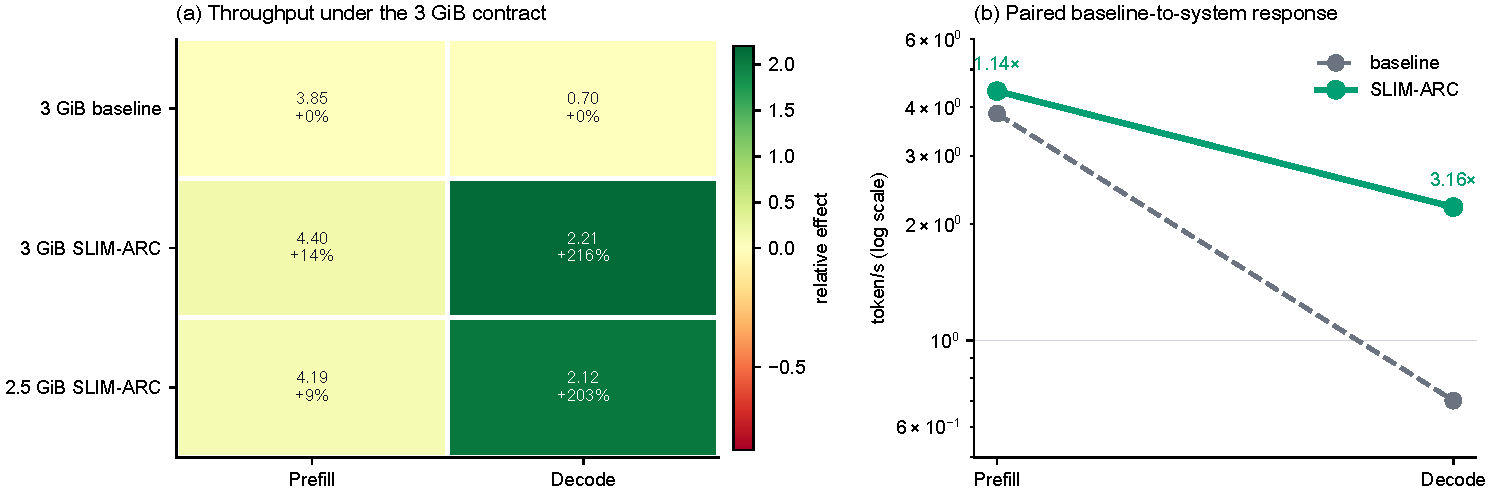
\includegraphics[width=0.98\textwidth]{figures/rk3588_3g_main.pdf}
\caption{RK3588 3\,GiB 主实验的归一化温度图与配对响应。}
\end{figure}

\paragraph{Raspberry Pi 5 慢存储实验。}
在 4\,GiB、运行期 no-swap 的 USB/FUSE 链路上，系统从扩大预取转向保留确定复用页。A28 的 shared expert 与 hot512 驻留相对 A24 将 Decode 从 0.055614 提高到 0.063486\,token/s，提升 14.16\%，wall time 从 547\,s 降至 511\,s。A29 将预算限制为 16\,MiB，在吞吐近似不变的同时将投机 weight I/O 降低 98.44\%。512\,MiB 跨 token LRU 最终达到 0.065856\,token/s 和 503\,s。

\begin{table}[H]
\centering
\small
\caption{Raspberry Pi 5 的慢存储策略演进}
\begin{tabular}{llrrr}
\toprule
编号 & 策略 & Prefill & Decode & Wall(s) \\
\midrule
A24 & no expert prefetch & 0.201104 & 0.055614 & 547.0 \\
A28 & shared + hot512 & 0.204023 & 0.063486 & 511.0 \\
A29 & A28 + 16\,MiB budget & 0.204283 & 0.063585 & 510.5 \\
A32 & no weight prefetch & 0.203642 & 0.065246 & 505.0 \\
A34 & 512\,MiB cross-token LRU & 0.203585 & \textbf{0.065856} & \textbf{503.0} \\
\bottomrule
\end{tabular}
\end{table}

\subsection{消融与专项实验}

\paragraph{阶段化页建议。}
RK3588 消融按阶段逐步切换访问建议，动态全 SEQUENTIAL 达到 Prefill 2.84、Decode 1.40\,token/s，说明页建议应与 Prefill/Decode 阶段以及实际存储介质共同选择。

\begin{figure}[H]
\centering
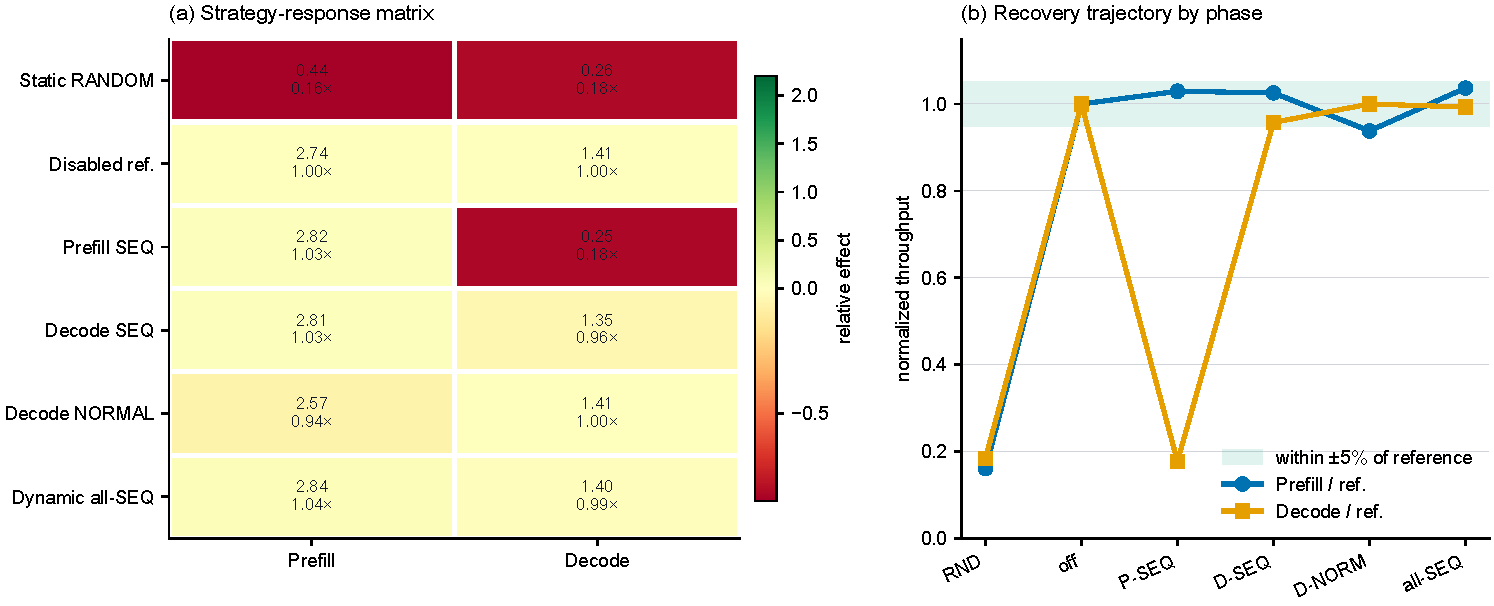
\includegraphics[width=0.98\textwidth]{figures/rk3588_dynamic_policy.pdf}
\caption{RK3588 阶段化页建议的策略响应图。}
\end{figure}

\paragraph{专家预测、门控与预算。}
RK3588 temporal predictor 准确率为 34.9\%；confidence gating 将 expert issued 从 27,836.7\,MB 降至 12,123.6\,MB，hit rate 从 31.05\% 提高到 55.35\%，Decode 保持约 1.9\,token/s。Mac A22 cross-layer Router Top2 命中率达到 88.56\%，Decode 提高 9.96\%，wall time 缩短 7.77\%。这些结果表明，预测质量必须与投机字节和端到端时延联合分析。

\paragraph{线程与 readahead。}
Mac 的 8/6 Prefill/Decode 线程配置使 Decode 提高 20.23\%、wall time 缩短 5.91\%。持续 256\,KiB readahead 配置使 Prefill 提高 13.39\%、Decode 提高 2.10\%、wall time 缩短 6.39\%。系统将这些参数保留为设备配置，而不是写死为全平台常量。

\paragraph{Attention 与长上下文。}
RK3588 Qwen3-4B 上 FlashAttention auto 的 Decode 为 6.90\,token/s。80B 长上下文实验在 8192--16384 context 下完成 KV eviction 路径验证；动态策略在 \texttt{p512/n128} 下达到 6.09/2.08\,token/s。KV 优化与权重页管理分别控制上下文工作集和模型工作集，并通过统一预算协同。

\subsection{结果总结}

实验表明，SLIM-ARC 的收益来自三条主线。第一，mmap、关闭不必要的 repack 与可控页缓存使超大模型能够在小内存边界内运行。第二，阶段化页建议和设备配置使访问模式贴合实际存储链路。第三，专家预测只有与预算、热度、事实结算和安全回收结合后，才能把 MoE 稀疏激活转化为可管理的工作集。RK3588 3\,GiB 与 Raspberry Pi 5 慢存储实验分别验证了强内存压力和高 I/O 代价下的策略选择。

\newpage
\section{总结与未来工作}

SLIM-ARC 构建了面向内存受限端侧设备的 MoE 推理运行时。系统以阶段识别为入口，用 mmap 与动态页建议控制普通权重访问，以 Router 反馈闭环控制专家页面，以压力、热度和统一预算协调驻留、回收与 KV cache，并通过模型所有权和租约机制保证后台调度与映射生命周期一致。

跨设备实验验证了系统的核心目标：WSL 8\,GiB 同合同实验将 80B Decode 从 0.08 提高到 0.43\,token/s，32\,GiB 热缓存区间通过 FlashAttention 达到 5.16\,token/s；48.41\,GB 模型可在 2\,GiB、no-swap 环境中完成推理；RK3588 3\,GiB 下 Decode 达到 2.21\,token/s；Raspberry Pi 5 上确定性专家驻留与严格 I/O 预算同时改善吞吐和 wall time。结果说明，端侧推理优化的关键不是孤立扩大预取，而是依据阶段、压力和介质构造受约束的工作集。

未来工作将继续研究更长上下文下的 KV 分层、多级存储上的专家放置、在线访问模型与异构计算协同，并扩大任务质量与多轮统计规模。系统将继续保持权重语义不变、策略可关闭、资源边界可观测的原则。

\newpage
\appendix
\section{主要实验数据汇总}

\begin{longtable}{p{0.16\textwidth}p{0.23\textwidth}p{0.20\textwidth}p{0.32\textwidth}}
\toprule
平台 & 模型与约束 & 配置 & 结果 \\
\midrule
x86/WSL & Qwen3-Next-80B，8\,GiB，pp4/tg1 & baseline $\rightarrow$ SLIM-ARC & Decode 0.08 $\rightarrow$ 0.43\,token/s，$+437.5\%$ \\
x86/WSL & Qwen3-Next-80B IQ4\_XS，16\,GiB & 8 threads & Decode $2.27\pm0.38$\,token/s \\
x86/WSL & Qwen3-Next-80B IQ4\_XS，32\,GiB & 8 threads & Prefill $4.44\pm1.53$，Decode $3.03\pm0.29$\,token/s \\
x86/WSL & 32\,GiB warm，KV q4\_0 & FA off $\rightarrow$ auto & Decode 3.01 $\rightarrow$ 5.16\,token/s，$+71.4\%$ \\
Mac/Colima & Qwen3-Next-80B，2\,GiB，4 vCPU，no-swap & A24，pp64/tg16 & Prefill 3.908455，Decode 0.709095\,token/s，wall 58.06\,s \\
RK3588 & Qwen3-Next-80B，3\,GiB，4 threads，swap 0 & baseline & Prefill 3.85，Decode 0.70\,token/s \\
RK3588 & 同上 & SLIM-ARC & Prefill 4.40，Decode 2.21\,token/s \\
RK3588 & 同上 & SLIM-ARC + KV & Prefill 4.19，Decode 2.12\,token/s \\
Raspberry Pi 5 & Qwen3-Next-80B，4\,GiB，USB/FUSE & A28 shared + hot512 & Prefill 0.204023，Decode 0.063486，wall 511\,s \\
Raspberry Pi 5 & 同上 & A29 16\,MiB budget & 投机 weight I/O 降低 98.44\% \\
Raspberry Pi 5 & 同上 & A34 cross-token LRU & Decode 0.065856，wall 503\,s \\
\bottomrule
\end{longtable}

\section{复现入口}

核心补丁位于 \texttt{patches/llama-upstream/}，\texttt{scripts/apply-slim-arc.py} 将模块应用到固定 llama.cpp 源码树。C++ 单元测试由 \texttt{tests/run-cpp-unit.sh} 执行；Mac 受限内存入口位于 \texttt{scripts/macos/}。实验复现应固定模型 SHA-256、llama.cpp 提交、内存与 swap 上限、线程数、Prompt/Generation 长度和缓存状态。

\begin{thebibliography}{20}
\bibitem{flexinfer} H. Du et al., ``FlexInfer: Breaking Memory Constraint via Flexible and Efficient Offloading for On-Device LLM Inference,'' EuroMLSys, 2025.
\bibitem{powerinfer2} Z. Xue et al., ``PowerInfer-2: Fast Large Language Model Inference on a Smartphone,'' 2024.
\bibitem{ktransformers} KTransformers, \url{https://github.com/kvcache-ai/ktransformers}.
\bibitem{flashattention} T. Dao et al., ``FlashAttention: Fast and Memory-Efficient Exact Attention with IO-Awareness,'' NeurIPS, 2022.
\bibitem{pagedattention} W. Kwon et al., ``Efficient Memory Management for Large Language Model Serving with PagedAttention,'' SOSP, 2023.
\bibitem{streamingllm} G. Xiao et al., ``Efficient Streaming Language Models with Attention Sinks,'' ICLR, 2024.
\bibitem{llamacpp} llama.cpp, \url{https://github.com/ggml-org/llama.cpp}.
\bibitem{cgroup} Linux kernel documentation, ``Control Group v2,'' \url{https://docs.kernel.org/admin-guide/cgroup-v2.html}.
\end{thebibliography}

\end{document}
